\documentclass[11pt]{amsart}
\usepackage{amsmath,amssymb,amsthm,mathtools,enumitem}
\usepackage[margin=1in]{geometry}
\usepackage{hyperref}
\usepackage{graphicx}
\graphicspath{{./}}

\newtheorem{theorem}{Theorem}[section]
\newtheorem{proposition}[theorem]{Proposition}
\newtheorem{corollary}[theorem]{Corollary}
\theoremstyle{remark}
\newtheorem*{remark}{Remark}

\title{The Cutting Plane: Every Line Through the Multiplication Table Is a Conic Section}
\author{Jeremy Ebert}
\address{Franklin County, Ohio, USA}
\date{2026}

\numberwithin{equation}{section}
\begin{document}
\pagestyle{plain}
\maketitle

\begin{abstract}
Write out the ordinary multiplication table and draw a straight line through it. What curve does that line trace, once the flat factor triangle is projected symmetrically onto the cone by the geometric-mean height? We classify the resulting sections completely: ellipse, parabola, nondegenerate hyperbola, or the corresponding degenerate generator section according to the line coefficients. Anti-diagonals give circles and individual rows or columns give parabolas. We also isolate an exact tangency between every row/column parabola and the anti-diagonal circle whose diameter equals the fixed factor level, and give the true semi-axes and eccentricity of the general ellipse section. The same coordinates restate Fermat factorization and reorganize the classical Dirichlet divisor summatory identity around nested diagonal gnomons.
\end{abstract}

\section{Introduction}
Figure~\ref{fig:table_line}(b) is the ordinary multiplication table written in the coordinates
\begin{equation}
X=\frac{x-y}{2},\qquad T=\frac{x+y}{2}.
\end{equation}
Every lattice cell still represents the ordinary product $xy$; the coordinate change merely turns the usual square arrangement into a triangular side view. Geometrically, this factor triangle sits in the plane $Y=0$. The outer boundary shown is $x+y=12$, and the dashed anti-diagonal $x+y=8$ passes through $(2,6),(4,4),(6,2)$.

There is also a classical geometric reason for the third coordinate. Given a rectangle with sides $x$ and $y$, place the two lengths end to end as the diameter of a semicircle and erect the perpendicular at their junction. The right-triangle altitude theorem gives the magnitude of that perpendicular as $\sqrt{xy}$. We therefore project each factor point normally from the flat triangle to both sides of the cone:
\begin{equation}
\Pi_\pm(x,y)=\left(\frac{x-y}{2},\ \pm\sqrt{xy},\ \frac{x+y}{2}\right).
\end{equation}
Equivalently, the fundamental relation is
\begin{equation}
X=\frac{x-y}{2},\qquad Y^2=xy,\qquad T=\frac{x+y}{2}.
\end{equation}
The radius, geometric-mean height, and signed offset satisfy
\begin{equation}
X^2+Y^2=T^2.
\end{equation}
Thus every positive factor pair has two symmetric cone images, exchanged by $Y\mapsto-Y$. For example, $(x,y)=(2,6)$ gives $(X,Y,T)=(-2,\pm\sqrt{12},4)$ and $4+12=16$. On the boundary $xy=0$ the two images coalesce at $Y=0$.

Anti-diagonals $x+y=K$ become fixed-$T$ circles. A general line $ax+by=c$ in the flat factor triangle becomes a cutting plane, and its two-sided projection traces the corresponding complete conic section on the cone. The reflected pair
\begin{equation}
8x+4y=32,\qquad 4x+8y=32
\end{equation}
is shown throughout Figure~\ref{fig:table_line} as a concrete example.

The emphasis here is deliberately geometric and elementary. Arithmetic structures that can subsequently act on this cone are treated in companion work; none is required for the results below.

\begin{remark}[Related work]
The classical analytic approach to the divisor summatory function proceeds via Vorono\"i summation and exponential sums \cite{Huxley1996,IwaniecKowalski2004}, where smoothing is routinely introduced to simplify the analysis \cite{BalkanovaDukeFrolenkov2026,BordellesDaval2026}. The present geometric viewpoint is complementary: it retains the discrete lattice structure that smoothing discards. A recent geometric re-reading of arithmetic functions in a similar spirit is \cite{Kobin2025}.
\end{remark}

\begin{figure}[ht]
\centering
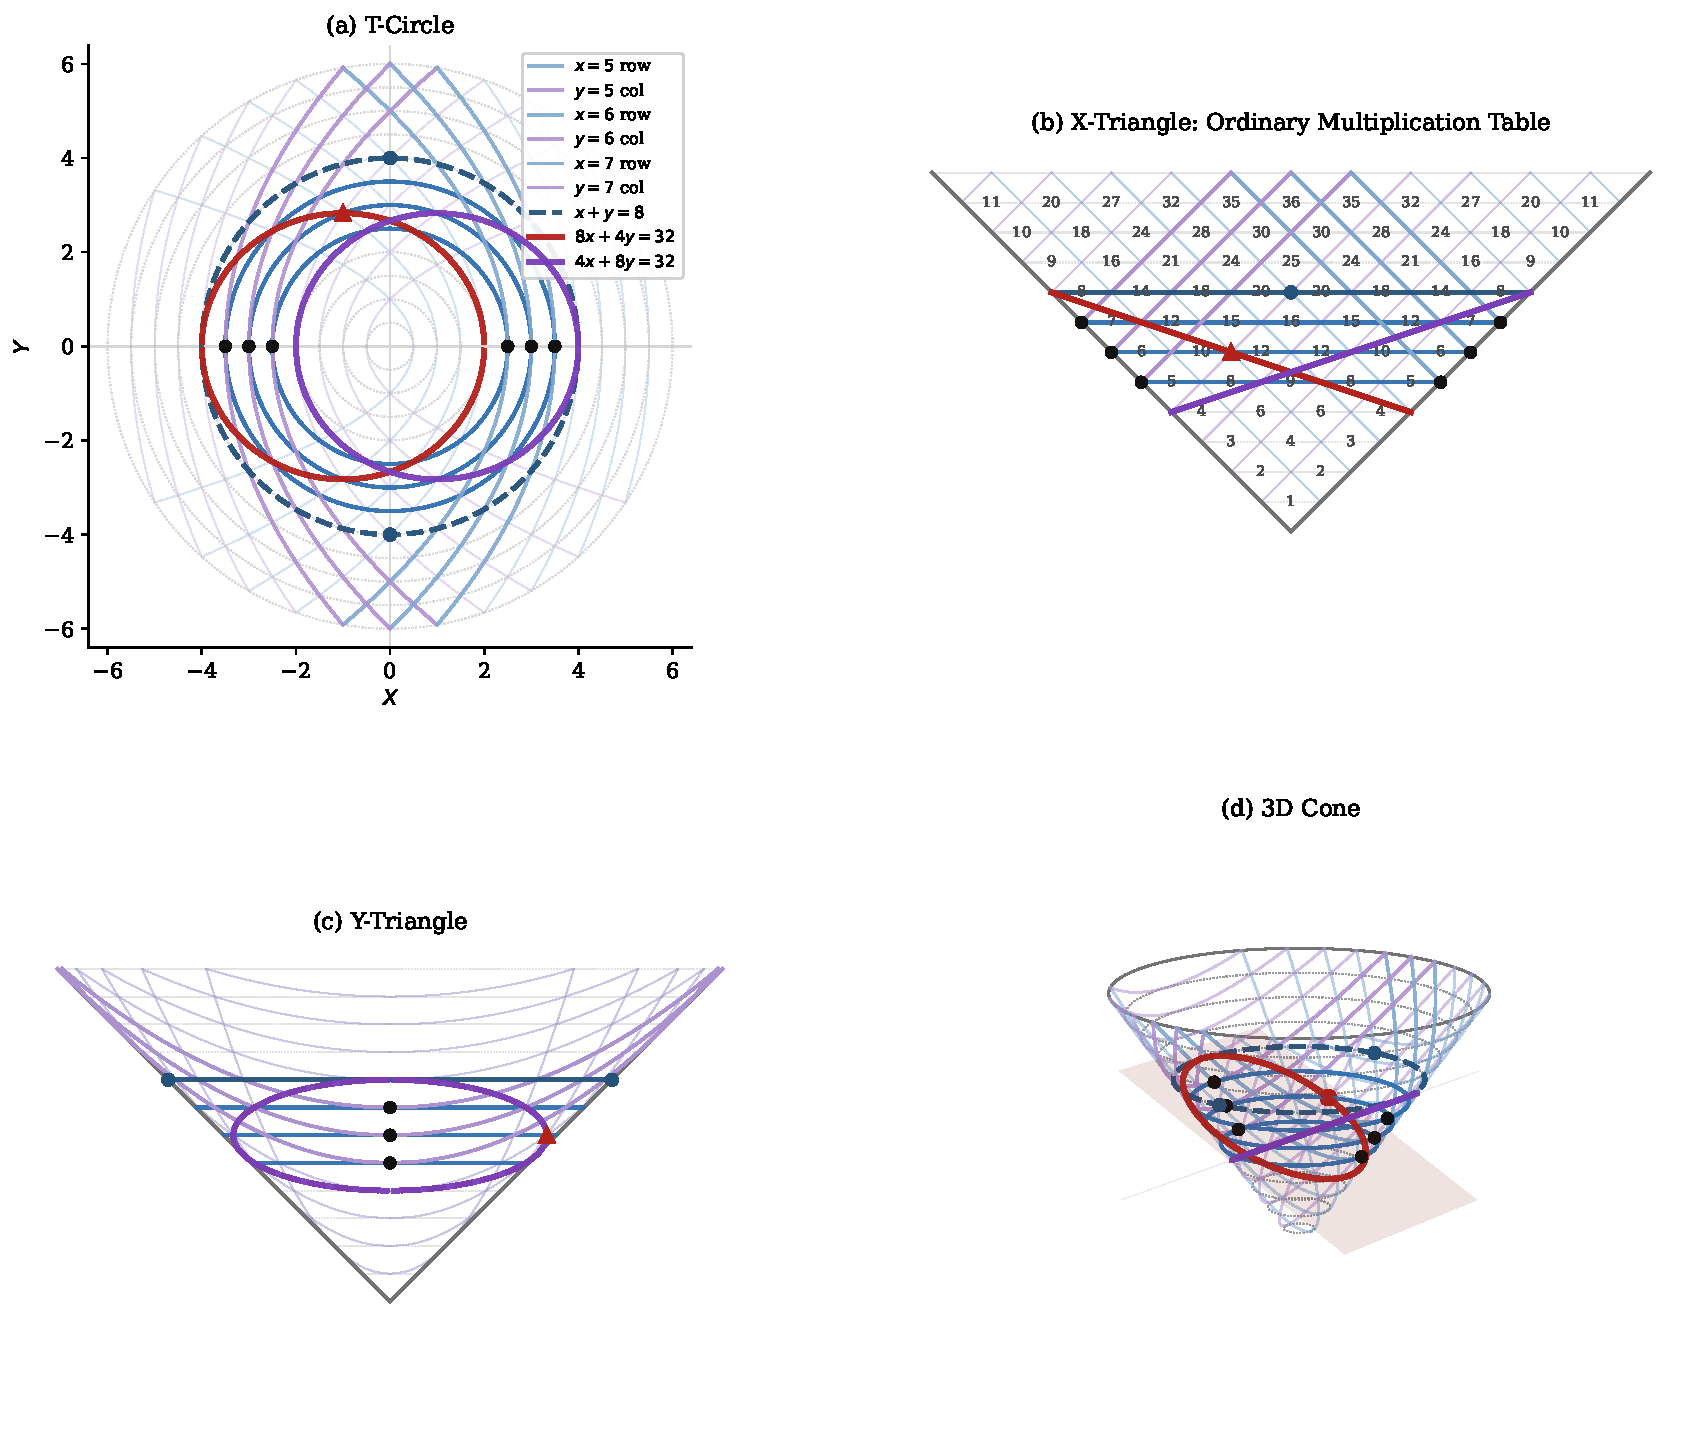
\includegraphics[width=\textwidth]{fig_cutting_plane_4panel.pdf}
\caption{Four views of the same factor geometry, bounded by $x+y=12$. (a) Fixed sums are concentric circles, row and column families are mirror parabolas, and the red/purple cuts are the mirror ellipses from $8x+4y=32$ and $4x+8y=32$; the dashed circle is $x+y=8$. (b) Side view in $(X,T)$, where the multiplication table is the flat triangular carrier at $Y=0$ and the cuts are straight lines. (c) Side view in $(Y,T)$: rows and columns coincide as a single parabola mesh, and the two mirror cuts project to the same $(Y,T)$ locus (dashed red over solid purple). (d) The two-sided geometric-mean projection onto $X^2+Y^2=T^2$, where the same cuts are literal plane sections. The figure is illustrative; the claims are proved below.}
\label{fig:table_line}
\end{figure}

\section{Mean-Value Coordinates and the Conic Identity}
For $x,y>0$ define the two-sided projection
\begin{equation}
\Pi_\pm(x,y)=\left(X,Y,T\right)=\left(\frac{x-y}2,\ \pm\sqrt{xy},\ \frac{x+y}2\right),\qquad Y^2=xy. 
\end{equation}
Then
\begin{equation}
X^2+Y^2=T^2. 
\end{equation}
The inverse factor coordinates are
\begin{equation}
x=T+X,\qquad y=T-X. 
\end{equation}
Thus the sign of $Y$ is geometric lift data: both signs encode the same factor pair. The involution
\begin{equation}
\iota_Y:(X,Y,T)\longmapsto(X,-Y,T)
\end{equation}
exchanges the two cone images while fixing $(x,y)$. Factor exchange $(x,y)\mapsto(y,x)$ is instead exactly $X\mapsto-X$ with $Y^2,T$ fixed. We use this convention throughout; in particular positive $X$ means $x>y$.

Fixing $x+y=K$ fixes $T=K/2$, giving the complete circle
\begin{equation}
X^2+Y^2=(K/2)^2.
\end{equation}
For integer $K\ge2$, each of the $K-1$ positive factor pairs $(x,K-x)$, $x=1,\ldots,K-1$, contributes its two symmetric points to this circle. In the complex coordinate $z=X+iY$, these two points are the conjugate pair
\begin{equation}
z_\pm=X\pm i\sqrt{xy},\qquad z_-=\overline{z_+},\qquad z\overline z=T^2.
\end{equation}
Equivalently,
\begin{equation}
z_+=\frac{(\sqrt{x}+i\sqrt{y})^2}{2},\qquad z_-=\frac{(\sqrt{x}-i\sqrt{y})^2}{2}.
\end{equation}
This is only the ordinary complex coordinate on a fixed-$T$ cutting circle; no arithmetic or cyclotomic identification is asserted here.

\section{The General Conic Theorem}
\begin{theorem}\label{thm:conic}
Let $a,b$ be real numbers, not both zero, and let $ax+by=c$ meet the positive factor quadrant. Under the two-sided projection (2.1), its cutting plane meets the cone $X^2+Y^2=T^2$ in an ellipse when $ab>0$, a parabola when $ab=0$, and a nondegenerate hyperbola when $ab<0$ and $c\ne0$. When $ab<0$ and $c=0$, the full algebraic section is the degenerate pair of cone generators; within the positive-factor branch the factor-domain section is the compatible generator ray, whose two lifts coalesce at $Y=0$. When $a=b\ne0$, the ellipse is a fixed-sum circle.
\end{theorem}
\begin{proof}
For $b\ne0$, $y=(c-ax)/b$, hence
\begin{equation}
Y^2=xy=\frac cbx-\frac abx^2.
\end{equation}
Because (2.1) includes both signs of $Y$, this quadratic relation gives the complete symmetric conic section rather than only its upper half. The sign of $-a/b$ gives the nondegenerate ellipse/parabola/hyperbola cases. If $ab<0$ and $c=0$, then
\begin{equation}
Y^2=-\frac ab x^2,
\end{equation}
which factors into two lines in the full algebraic cone section; restricting to the positive factor domain retains the compatible generator ray. The cases $a=0$ or $b=0$ are the row/column parabolas below. If $a=b\ne0$, then $x+y=c/a$ is constant.
\end{proof}

\begin{proposition}[Rows and columns]\label{prop:rows}
With the convention $X=(x-y)/2$, a fixed row $x=u$ satisfies
\begin{equation}
X+T=u,\qquad Y^2=u(T-X)=u^2-2uX,
\end{equation}
while a fixed column $y=u$ satisfies
\begin{equation}
T-X=u,\qquad Y^2=u(T+X)=u^2+2uX.
\end{equation}
These are complete parabolas because both signs of $Y$ are present. The row and column families are exchanged by $X\mapsto-X$.
\end{proposition}

\begin{proof}
For $x=u$, equations (2.3) give $T+X=u$ and $y=T-X$, hence $Y^2=xy=u(T-X)$. The column identity is the factor-exchange reflection. In three dimensions the row plane $T+X=u$ is parallel to the cone generator $(-1,0,1)$, and the column plane $T-X=u$ is parallel to $(1,0,1)$, giving the classical plane-section characterization of a parabola.
\end{proof}

\begin{proposition}[Anti-diagonal tangency]\label{prop:tangent}
For every $u>0$, the row and column parabolas at factor level $u$ are tangent in the $(X,Y)$ projection to
\begin{equation}
C_{u/2}:\quad X^2+Y^2=(u/2)^2.
\end{equation}
The row $x=u$ is tangent at $(X,Y)=(u/2,0)$, and the column $y=u$ at $(-u/2,0)$. On the cone these are $(T,X,Y)=(u/2,\pm u/2,0)$.
\end{proposition}
\begin{proof}
The row parabola $Y^2=u^2-2uX$ has vertex $(u/2,0)$; the column parabola $Y^2=u^2+2uX$ has vertex $(-u/2,0)$. Both vertices lie on $C_{u/2}$, and implicit differentiation gives the same vertical tangent there. The signs also follow directly from (2.3): at the row endpoint $y=0$, $X=x/2=u/2$; at the column endpoint $x=0$, $X=-y/2=-u/2$.
\end{proof}

\begin{remark}
Factor level $u$ corresponds exactly to tangent-circle radius $T=u/2$. A factor mesh of spacing $1/m$ therefore induces a tangent-circle radius mesh of spacing $1/(2m)$. This is a geometric statement, not an arithmetic invariance claim.
\end{remark}

For the metric statements about an ellipse, multiplying the line equation by $-1$ if necessary lets us normalize the nonempty positive-quadrant case to $a,b,c>0$ without changing the geometric line.

\begin{proposition}[Coordinate maximum of an ellipse]\label{prop:semiaxes}
Assume $a,b,c>0$. Then $Y^2$ is maximized at
\begin{equation}
x=\frac{c}{2a},\qquad y=\frac{c}{2b},
\end{equation}
and
\begin{equation}
Y_{\max}^2=\frac{c^2}{4ab}.
\end{equation}
\end{proposition}
\begin{proof}
Differentiate $Y^2=(c/b)x-(a/b)x^2$ and substitute the critical point; the line equation then gives the stated $y$ coordinate.
\end{proof}

For $8x+4y=32$, the maximum is $(x,y)=(2,4)$ with $Y^2_{\max}=8$. Since $X=(x-y)/2$, this point has $(X,T)=(-1,3)$. Its reflected cut $4x+8y=32$ has maximum $(4,2)$ and $(X,T)=(1,3)$. This fixes the red/purple orientation independently of the drawing.

\begin{proposition}[True ellipse axes and eccentricity]\label{prop:trueaxes}
Assume $a,b,c>0$. The ellipse cut from the cone by $ax+by=c$ has semi-minor axis
\begin{equation}
b_{\rm semi}=\frac{c}{2\sqrt{ab}},
\end{equation}
semi-major axis
\begin{equation}
a_{\rm semi}=\frac{c\sqrt{2(a^2+b^2)}}{4ab},
\end{equation}
and eccentricity
\begin{equation}
e=\frac{|a-b|}{\sqrt{a^2+b^2}}.
\end{equation}
Thus eccentricity depends only on $a/b$, and $e=0$ exactly when $a=b$.
\end{proposition}
\begin{proof}
The section is symmetric under $Y\mapsto-Y$, and the $Y$ direction lies in the cutting plane. Its $Y$ semi-axis is therefore $Y_{\max}=c/(2\sqrt{ab})$. At $Y=0$ the two endpoints are
\begin{equation}
\left(\frac{c}{2a},0,\frac{c}{2a}\right),\qquad
\left(-\frac{c}{2b},0,\frac{c}{2b}\right).
\end{equation}
The direction joining these endpoints is orthogonal to the $Y$ direction, so half their Euclidean distance is the other semi-axis, namely
\begin{equation}
\frac{c\sqrt{2(a^2+b^2)}}{4ab}.
\end{equation}
Moreover
\begin{equation}
\frac{a_{\rm semi}^2}{b_{\rm semi}^2}=\frac{a^2+b^2}{2ab}\ge1,
\end{equation}
so these are indeed the major and minor axes. Finally $e^2=1-b_{\rm semi}^2/a_{\rm semi}^2=(a-b)^2/(a^2+b^2)$.
\end{proof}

For $8x+4y=32$,
\begin{equation}
a_{\rm semi}=\sqrt{10},\qquad b_{\rm semi}=2\sqrt2,\qquad e=1/\sqrt5.
\end{equation}

\section{Constant Products: Fermat Factorization and the Divisor Summatory}
Fixing $xy=N$ fixes $Y^2=N$, so the two cone images lie in the parallel planes
\begin{equation}
Y=\pm\sqrt N,
\end{equation}
while their common side-view projection satisfies
\begin{equation}
T^2-X^2=N.
\end{equation}
This hyperbola is the bridge to two classical applications.

For odd $N$, Fermat's method searches integers $T\ge\lceil\sqrt N\rceil$ until $T^2-N=X^2$, at which point
\begin{equation}
N=(T-X)(T+X).
\end{equation}
Thus the constant-product hyperbola records the same factorization search directly in mean-value coordinates, and its two-sided cone projection is the reflected pair $Y=\pm\sqrt N$.

The same boundary organizes the divisor summatory function. Let
\begin{equation}
D(n)=\sum_{k=1}^n d(k)=\#\{(x,y)\in\mathbb Z_{\ge1}^2:xy\le n\}.
\end{equation}
For each diagonal vertex $(u,u)$, $1\le u\le\lfloor\sqrt n\rfloor$, the horizontal and vertical arms terminate at the constant-product boundary. Their integer arm length is $\lfloor n/u\rfloor-u$. Hence
\begin{equation}
D(n)=\sum_{u=1}^{\lfloor\sqrt n\rfloor}\left[2\left(\left\lfloor\frac nu\right\rfloor-u\right)+1\right], 
\end{equation}
and therefore
\begin{equation}
D(n)=2\sum_{u=1}^{\lfloor\sqrt n\rfloor}\left\lfloor\frac nu\right\rfloor-\lfloor\sqrt n\rfloor^2. 
\end{equation}
This is the classical symmetric Dirichlet hyperbola identity, read as nested gnomons whose arms are pieces of the row/column parabolas cut off by $xy=n$.

For $n=11$, the smallest integer anti-diagonal bounding the whole positive divisor region is $x+y=12$. The triangular region $x+y\le12$ contains
\begin{equation}
T_{11}=1+2+\cdots+11=66
\end{equation}
positive lattice cells. Within it,
\begin{equation}
D(11)=29,\qquad A_{11}:=T_{11}-D(11)=37\ \text{(OEIS A161664)}.
\end{equation}
The constant-product boundary is
\begin{equation}
xy=11\iff Y^2=11\iff T^2-X^2=11,
\end{equation}
so its two cone images lie in $Y=\pm\sqrt{11}$. It meets $x+y=12$ at $(1,11)$ and $(11,1)$, corresponding to $(X,T)=(-5,6)$ and $(5,6)$.

\begin{figure}[ht]
\centering
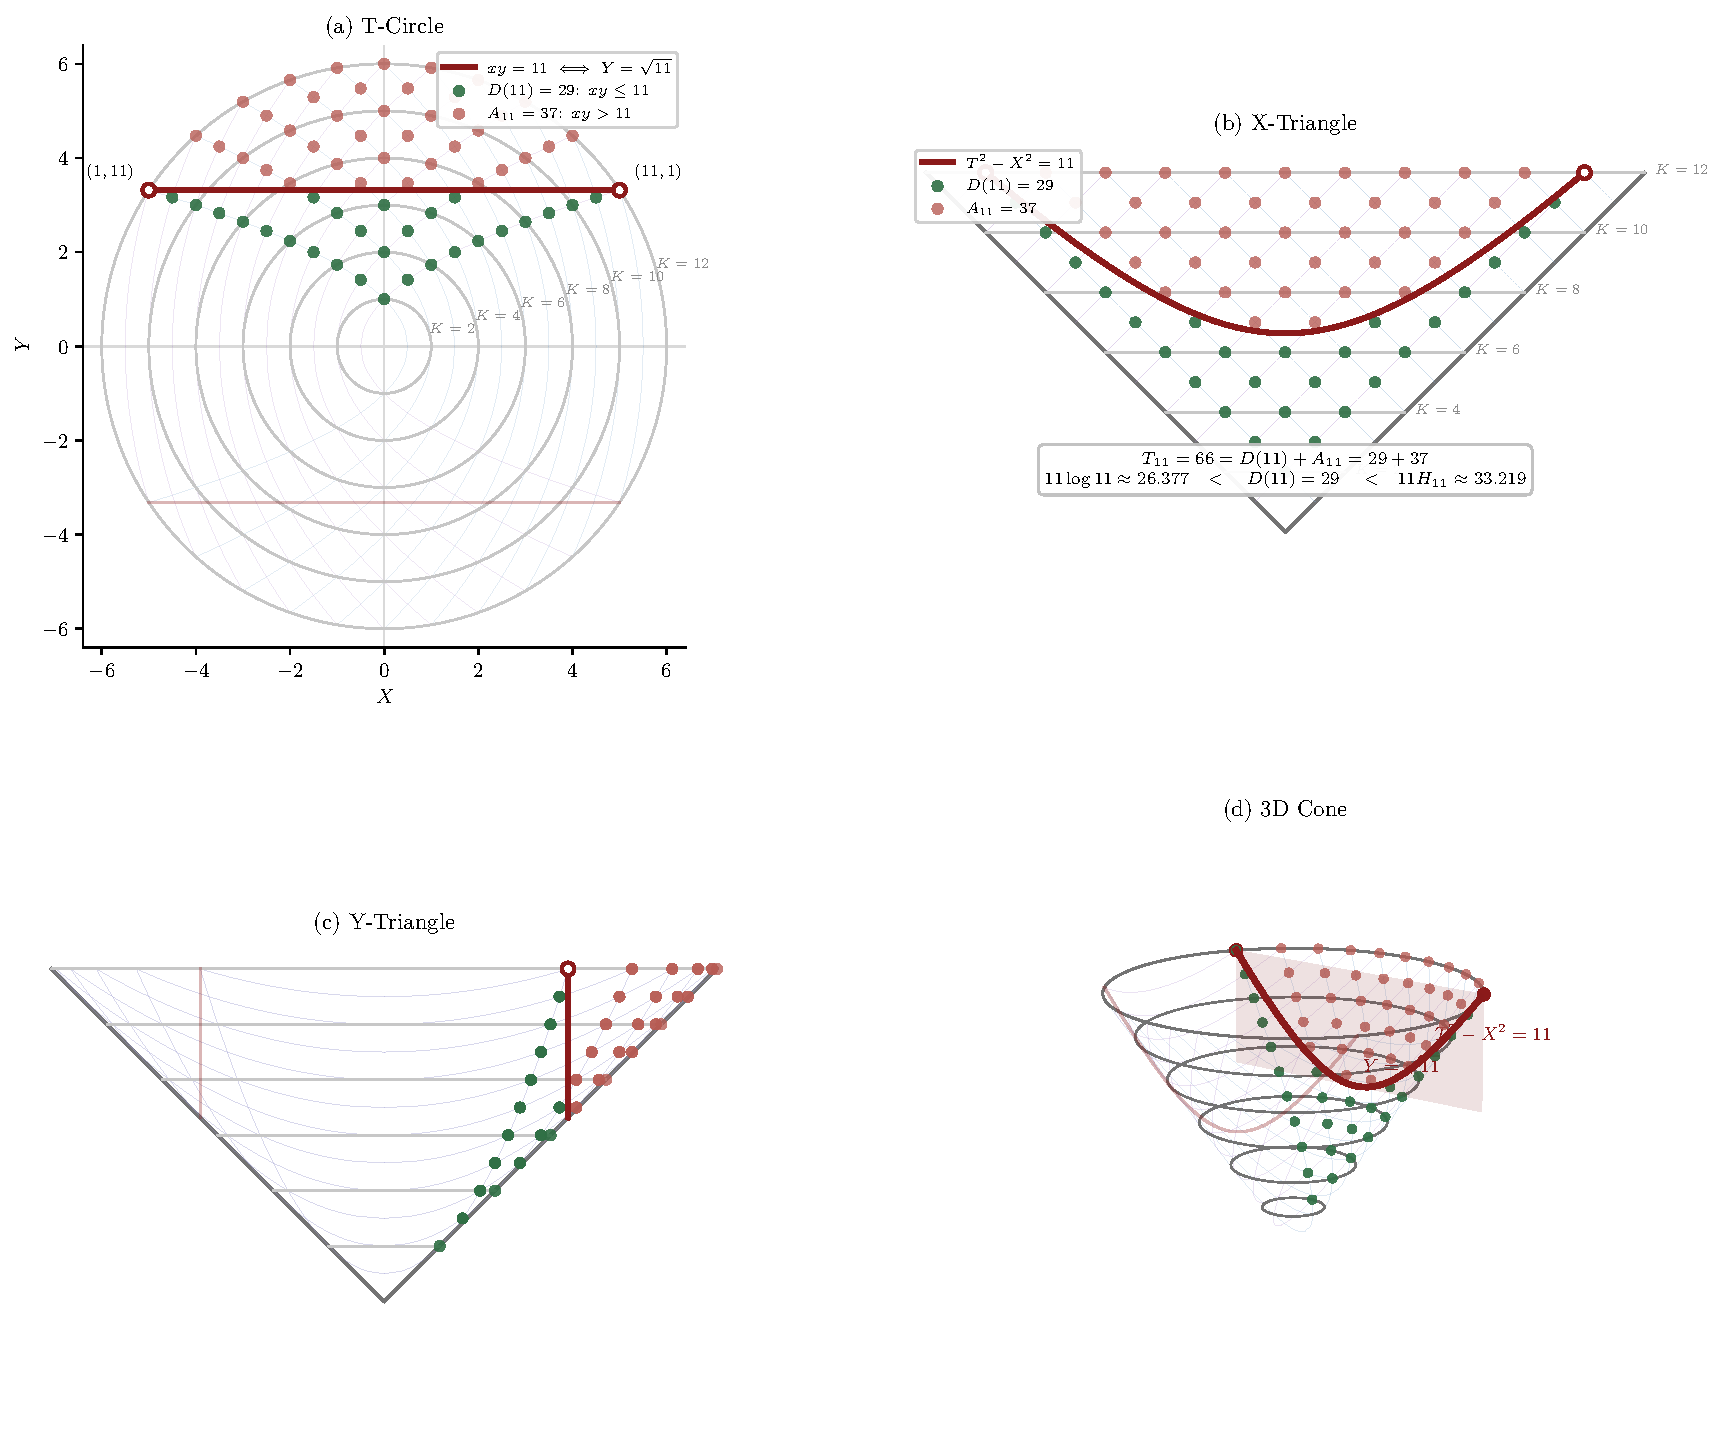
\includegraphics[width=\textwidth]{fig_divisor_summatory_11_4panel.pdf}
\caption{The divisor summatory geometry for $n=11$ in the same four views as Figure~\ref{fig:table_line}. The $66$ cells inside $x+y\le12$ split exactly into $D(11)=29$ (green, $xy\le11$) and the triangular complement $A_{11}=37$ (red, $xy>11$), shown on the upper lift $Y=+\sqrt{xy}$. The boundary $xy=11$ has the two cone images $Y=\pm\sqrt{11}$: a horizontal secant in (a), the hyperbola $T^2-X^2=11$ in (b), and a vertical secant in the $(Y,T)$ view (c). The displayed $11\log11$ and $11H_{11}$ values (where $H_{11}=1+\frac12+\cdots+\frac1{11}$ is the $11$th harmonic number) are comparison quantities only; they are not asserted to equal the discrete count.}
\label{fig:divisor11}
\end{figure}

The choice $n=11$ is illustrative rather than structural: the identities above hold for general $n$. It is useful here because the extremal factor pairs lie exactly on $x+y=12$.

\section{Discussion}
The cone identity organizes three elementary structures on one carrier: the flat multiplication triangle in $Y=0$ projects symmetrically to the cone, linear conditions become complete conic sections, constant products become reflected $Y$-levels with a common Lorentz-type side-view hyperbola, and the divisor summatory region decomposes into diagonal gnomons. Proposition~\ref{prop:tangent} adds an exact bridge: each fixed factor level determines both a row/column parabola and a unique tangent anti-diagonal circle of radius $u/2$.

The two basic reflections are distinct. Factor exchange is $X\mapsto-X$ and exchanges rows with columns. The cone-lift involution is $Y\mapsto-Y$ and exchanges the two geometric images of the same factor pair. On every fixed-$T$ circle the latter is ordinary complex conjugation in $z=X+iY$. This geometric conjugation is exact, but no identification with a later arithmetic or cyclotomic conjugation is made in this paper.

This is the natural stopping point for the geometric paper. Later arithmetic or operator constructions may use the same cone and its two generator rays, but they should be cited as companion results rather than imported into these elementary proofs.

\section*{Acknowledgment}
Large language model tools were used for drafting, figure preparation, and checking.

\begin{thebibliography}{9}
\bibitem{Dickson} L.~E.~Dickson, \emph{History of the Theory of Numbers, Vol.~I}, Carnegie Institution, 1919, Ch.~14.
\bibitem{Dirichlet} P.~G.~L.~Dirichlet, \"Uber die Bestimmung der mittleren Werthe in der Zahlentheorie, \emph{Abh. K\"onigl. Preuss. Akad. Wiss.} (1849), 69--83.
\bibitem{Huxley1996} M.~N.~Huxley, \emph{Area, Lattice Points, and Exponential Sums}, London Math.\ Soc.\ Monographs (N.S.) 13, Clarendon Press, Oxford, 1996.
\bibitem{IwaniecKowalski2004} H.~Iwaniec and E.~Kowalski, \emph{Analytic Number Theory}, Amer.\ Math.\ Soc.\ Colloq.\ Publ.\ 53, Providence, 2004.
\bibitem{BalkanovaDukeFrolenkov2026} O.~Balkanova, W.~Duke, and D.~Frolenkov, \emph{A Diophantine divisor problem and Hecke zeta functions}, Selecta Math.\ (2026), Art.~67.
\bibitem{BordellesDaval2026} O.~Bordell\`es and F.~Daval, \emph{On a smoothed Dirichlet divisor problem}, arXiv:2601.01905 [math.NT] (2026).
\bibitem{Kobin2025} A.~Kobin, \emph{Arithmetic functions and geometry}, arXiv:2504.13328 [math.NT] (2025).
\end{thebibliography}
\end{document}
